\begin{frame}
  \frametitle{1. Orbite relativamente compatte o iterate compattamente divergenti}
  \only<1-6>{\begin{block}{Teorema (Abate, 1991)}\begin{itshape}
    Sia $X$ una varietà taut e consideriamo $f \in \textnormal{Hol}(X,X)$. Le seguenti affermazioni sono equivalenti:\pause
    \begin{enumerate}
        \item la successione $\{f^k\}_{k \in \mathbb{N}}$ delle iterate di $f$ non è compattamente divergente;\pause
        \item la successione $\{f^k\}_{k \in \mathbb{N}}$ delle iterate di $f$ non contiene alcuna sottosuccessione compattamente divergente;\pause
        \item la successione $\{f^k\}_{k \in \mathbb{N}}$ delle iterate di $f$ è relativamente compatta in $\textnormal{Hol}(X,X)$;\pause
        \item l'orbita di $z$ è relativamente compatta in $X$ per ogni $z \in X$;\pause
        \item esiste $z_0 \in X$ la cui orbita è relativamente compatta in $X$.
    \end{enumerate}
  \end{itshape}\end{block}}
  \only<7-9>{\begin{ex}
    La palla unitaria in $\mathbb{C}^2$ meno l'origine è Kobayashi-iperbolica e $(\lambda,\kappa)$-visibile per ogni $\lambda\ge 1$ e $\kappa\ge 0$, ma non è taut. \setcounter{beamerpauses}{7}\pause La funzione $f(z,w)=(z/2,e^{i\theta}w)$ è un esempio che mostra come l'ipotesi taut sia indispensabile nel teorema di Abate. \pause Inoltre, mostra anche che è indispensabile nel teorema di tipo ``Wolff-Denjoy''.
  \end{ex}}
\end{frame}

\begin{frame}[t]
  \frametitle{2. Convergenza a una costante a meno di sottosuccessioni}
  \only<1-8>{
    \begin{block}{Lemma 1}\begin{itshape}
      Sia $X$ una sottovarietà complessa, connessa e relativamente compatta di una varietà complessa $Y$. \pause Supponiamo che esista $\kappa_0>0$ tale che $X$ sia $(1,\kappa_0)$-visibile. \pause Siano $Z$ una varietà Kobayashi-iperbolica e $\{f_n\}_{n\in\mathbb{N}}\subseteq\textnormal{Hol}(Z,X)$ una successione compattamente divergente. \pause Allora esistono $\xi\in\partial_YX$ e una sottosuccessione $\{f_{n_j}\}_{j\in\mathbb{N}}$ tali che $f_{n_j}(z)\longrightarrow\xi$ per ogni $z\in Z$.
  \end{itshape}\end{block}
  \only<5-8>{\textit{Traccia della dimostrazione:}} \only<5-6>{per assurdo, troviamo (a meno di sottosuccessioni) $z_0,z_1\in Z$ con $k_Z(z_0,z_1)<\kappa_0/2$ e $f_n(z_0)\longrightarrow\xi_0, f_n(z_1)\longrightarrow\xi_1$, dove $\xi_0,\xi_1\in\partial_YX$ e $\xi_0\not=\xi_1$.\setcounter{beamerpauses}{5}\pause

  Le varietà Kobayashi-iperboliche sono connesse da $(1,\kappa)$-simil-geodetiche per $\kappa>0$, quindi prendiamone una $\sigma:[0,T]\longrightarrow Z$ per $\kappa=\kappa_0/2$ con $\sigma(0)=z_0,\sigma(T)=z_1$.}
  \only<7-8>{Si verifica che le curve $f_n\circ\sigma$ sono $(1,\kappa_0)$-simil-geodetiche. \setcounter{beamerpauses}{7}\pause Per visibilità, esiste un compatto $K$ tale che
  $$\emptyset\not=K\cap f_n\big(\sigma([0,T])\big)$$
  per ogni $n$, ma $\sigma([0,T])$ è compatto e $\{f_n\}_{n\in\mathbb{N}}$ è compattamente divergente, contraddizione.\qed}
  }
  \only<9-12>{
    \begin{block}{Lemma 2}\begin{itshape}
      Sia $X$ una sottovarietà Kobayashi-iperbolica e relativamente compatta di una varietà complessa $Y$. \setcounter{beamerpauses}{9}\pause Supponiamo che esista $\kappa_0>0$ tale che $X$ sia $(1,\kappa_0)$-visibile. Sia $F\in\textnormal{Hol}(X,X)$ tale che la successione $\{F^n\}_{n\in\mathbb{N}}$ sia compattamente divergente.\pause
      
      Supponiamo che esistano un compatto $K\subseteq X$, una funzione strettamente crescente $\mu:\mathbb{N}\longrightarrow\mathbb{N}$ e $\xi\in\partial_YX$ tali che la successione $\{F^{\mu(j)}\}_{j\in\mathbb{N}}$ converge alla costante $\xi$ uniformemente su $K$. \pause Allora la successione $\{F^{\mu(j)}\}_{j\in\mathbb{N}}$ converge alla costante $\xi$ uniformemente sui compatti.
  \end{itshape}\end{block}}
  \only<13-22>{\textit{Traccia della dimostrazione:} sia $\xi$ dato dal Lemma 1 applicato a $\{F^{\mu(j)}\}_{j\in\mathbb{N}}$. \setcounter{beamerpauses}{13}\pause Supponiamo per assurdo che esistano un intorno $U$ di $\xi$, un compatto $H$ di $X$, una sottosuccessione $\{j_n\}_{n\in\mathbb{N}}$ e degli $z_n\in H$ tali che:\pause
  \begin{itemize}
    \item si ha $F^{\mu(j_n)}(z_n)\not\in U$ per ogni $n\in\mathbb{N}$;\pause
    \item si ha $z_n\longrightarrow\tilde{z}\in H$;\pause
    \item si ha $F^{\mu(j_n)}(z_n)\longrightarrow\xi'\in\partial_YX$;\pause
    \item si ha $F^{\mu(j_n)}(\tilde{z})\longrightarrow\xi''$.
  \end{itemize}\pause
  A meno di prendere prima una sottosuccessione che converga puntualmente a $\xi$ su tutta $X$, abbiamo $\xi''=\xi$. \pause Poiché $F^{\mu(j_n)}(z_n)\not\in U$ per ogni $n$, abbiamo $\xi'\not=\xi$. \pause Infine,
  $$k_X\big(F^{\mu(j_n)}(z_n),F^{\mu(j_n)}(\tilde{z})\big)\le k_X(z_n,\tilde{z})\longrightarrow 0;$$\pause
  si può dimostrare che, sotto condizioni di visibilità, questo non è possibile per successioni che tendono a punti distinti del bordo. \qed
  }
\end{frame}

\begin{frame}
  \frametitle{Caso non relativamente compatto}
  \only<1-2>{
    \begin{ex}
      Consideriamo $Y=\mathbb{C}, X=\{0<\mathfrak{Im}z<1\}$ e $F(z)=z+1$ o $F(z)=z-1$.\\

      \pause\begin{center}
        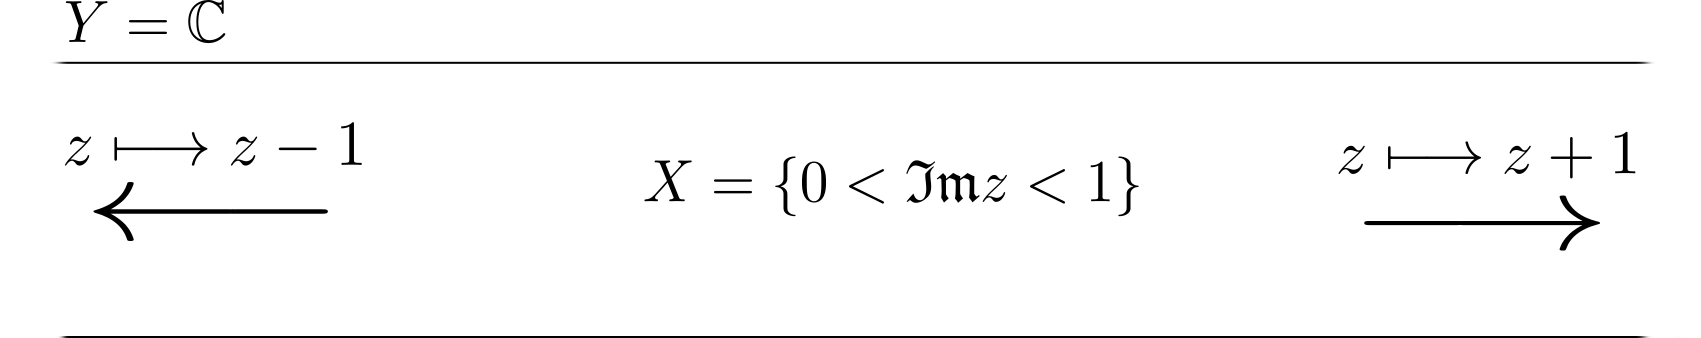
\includegraphics[width=0.8\textwidth]{esempio.png}
      \end{center}
    \end{ex}
  }
  \only<3-9>{
    \begin{defn}
      Sia $X$ uno spazio topologico non compatto. \setcounter{beamerpauses}{3}\pause Una \textit{fine} di $X$ è una funzione $e$ con dominio $\{K\subseteq X\mid K\text{ è compatto}\}$ tale che:\pause
      \begin{enumerate}
        \item a ogni compatto $K\subseteq X$ associa una componente connessa non vuota di $X\setminus K$;\pause
        \item per ogni coppia di compatti $K_1\subseteq K_2\subseteq X$ si ha $e(K_2)\subseteq e(K_1)$.\pause
      \end{enumerate}
    Indichiamo con $\mathcal{E}(X)$ l'insieme di tutte le fini di $X$.
  \end{defn}
  \pause
  \begin{prop}
    Sia $X$ uno spazio topologico connesso, localmente connesso, localmente compatto, di Hausdorff e che ammette un'esaustione in compatti. \pause
    
    Allora $X^\mathcal{E}=X\cup\mathcal{E}(X)$ ammette una topologia che lo rende una compattificazione di $X$.
\end{prop}
  }
  \only<10->{
    Problema: se $X$ è sottovarietà di $Y$, non sempre $\overline{X}$ è localmente connessa.\setcounter{beamerpauses}{10} \pause
    \begin{block}{Teorema (Bharali, Zimmer, 2022)}\begin{itshape}
      Sia $X$ una sottovarietà taut di una varietà complessa $Y$. \pause Supponiamo che $\overline{X}$ sia localmente connessa e che esista $\kappa_0>0$ tale che $X$ sia $(1,\kappa_0)$-ultravisibile. \pause
    
    Sia $F:X \longrightarrow X$ una funzione olomorfa. Allora vale esattamente una delle seguenti affermazioni:\pause
      \begin{enumerate}
        \item le orbite dei punti di $X$ tramite $F$ sono relativamente compatte in $X$; \pause oppure,
        \item esiste un unico punto $\xi\in\partial^\mathcal{E}X$ tale che la successione delle iterate di $F$ converge alla costante $\xi$ in $C^0(X,\overline{X}^\mathcal{E})$.
      \end{enumerate}
    \end{itshape}\end{block}
  }
  \pause
  Domanda: ultravisibilità implica locale connessione della chiusura?
\end{frame}

\begin{frame}
  \frametitle{Fine}
  \begin{center}
    \LARGE Grazie per l'attenzione!
  \end{center}
\end{frame}

\begin{frame}
  \frametitle{Bibliografia principale}
  \begin{thebibliography}{widest entry}
    \bibitem[A]{A} M. Abate: Iteration theory, compactly divergent sequences and commuting holomorphic maps. \textit{ Ann. Scuola Norm. Sup. Pisa Cl. Sci. Serie IV}, \textbf{18} (1991), no. 2, 167--191
    \bibitem[BM]{BM} G. Bharali, A. Maitra: A weak notion of visibility, a family of examples, and Wolff-Denjoy theorems. \textit{ Ann. Sc. Norm. Super. Pisa Cl. Sci. Serie V}, \textbf{22} (2021), no. 1, 195--240
    \bibitem[BZ1]{BZ1} G. Bharali, A. Zimmer: Goldilocks domains, a weak notion of visibility, and applications. \textit{ Adv. Math.}, \textbf{310} (2017), 377--425
    \bibitem[BZ2]{BZ2} G. Bharali, A. Zimmer: Unbounded visibility domains, the end compactification, and applications. Preprint, arXiv:2206.13869v1 (2022)
    \bibitem[CMS]{CMS} V. S. Chandel, A. Maitra, A. D. Sarkar: Notions of Visibility with respect to the Kobayashi distance: Comparison and Applications. Preprint, arXiv:2111.00549v1 (2021)
  \end{thebibliography}
\end{frame}